%   Filename    : chapter_1.tex 
\chapter{Introduction}
\label{sec:researchdesc}    %labels help you reference sections of your document

\section{Overview of the Current State of Technology}
\label{sec:overview}

This section gives the reader an overview of the specific technology or field in the international or
local setting. 
The information regarding the technology or field should be contemporary and not based on outdated sources. 
Discussion must not be too technical or too detailed.
   
\textcolor{red}{This section ends with a discussion on the problem/s faced by or that still exist in the specific
technology or field (e.g., limitations of existing software or algorithms). 
The problem statement would lead to the research objectives.}


It is   easy to include a figure in JPG or PNG format as shown in the  following example.  
Make sure that you explain what the figure is all about, and that you refer to your figure.  
For example, \figref{fig:disneystock} shows a graph of the performance of Disney stock from the 1980s to 2012.
  
%--- the following example shows how to include a figure in PNG format
\begin{figure}[t]                %-- use [t] to place figure at top, [b] to place at the bottom, [h] for here
   \centering                    %-- use this to center the figure
   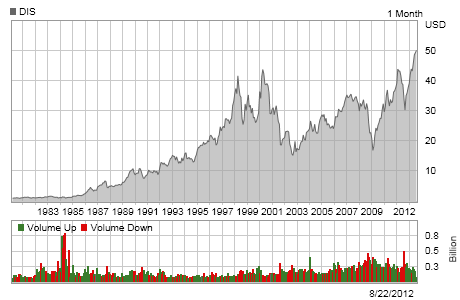
\includegraphics{DisneyChart.png}      %-- include image file named as "disneychart.png" 
   \caption{This is the figure's caption -- Disney stock chart.
   	Captions should fully describe the figure in a concise manner  such that there is not need to refer to the text when figuring out the graphic.}
    \label{fig:disneystock}
\end{figure}


Some notes on citing references.   
When using APA format, the author-date method of citation is  followed.   
This means that the author's last name and the year of publication for the source should  appear in the text, and a complete reference should appear in the reference list.

% Examples:
%     	Smith (1970) compared reaction times . . .
%     	In a recent study of reaction times (Smith, 1970), . . .   
%     	In 1970, Smith compared reaction times . . .
%	    Smith, et al., (1970) compared reaction times . . .
%     	In a recent study of reaction times (Smith, et al., 1970), . .
%     	In 1970, Smith, et al., compared reaction times . . .

Here are some examples on how to do the referencing (note author's name and years are different from commented examples).  
For APA citation details, refer to \url{http://www.ctan.org/tex-archive/biblio/bibtex/contrib/apacite/}. 

\begin{itemize}
 \item \citeA{kartch:2000:ERA} compared reaction times...
 \item In a recent study of reaction times \cite{kartch:2000:ERA}...
 \item In \citeyearNP{kartch:2000:ERA}, \citeauthor{kartch:2000:ERA} compared reaction times...
 \item \shortciteA{fedkiw:2001:VSO} compared reaction times... 
 \item In a recent study of reaction times \cite{fedkiw:2001:VSO}...
 \item In \citeyearNP{fedkiw:2001:VSO}, \shortciteauthor{fedkiw:2001:VSO}, compared reaction times...
\end{itemize}

The following are references from journal articles \cite{Park:2006:DSI, Pellacini:2005:LAH, sako:2001:SSB}.
 Here's an MS thesis document \cite{yee:2000:SSA}, and this is from PhD dissertation \cite{kartch:2000:ERA}. 
 For a book, reference is given as  \cite{parke:1996:CFA}. 
 Proceedings from a conference samples are \cite{Jobs95, fedkiw:2001:VSO, levoy:2000:TDM}.  
 The sample bibliography file named \textbf{myreferences.bib} is from the SIGGRAPH \LaTeX{}  template.  
 You can use a text editor to view the contents of the bib file.  
 It is your task to create your own bibliography file.  
 For those who downloaded papers from ACM or IEEE sites, there is a BibTeX link that you can click; thereafter, you just simply need to copy and paste the BibTeX entry into your own bibliography file.

The following shows how to include a program source code (or algorithm).  
The verbatim environment, as the name suggests, outputs text (including white spaces) as is...

\begin{verbatim}
               #include <stdio.h>
               main()
               {
                    printf("Hello world!\n");
               }
\end{verbatim}

\section{Problem Statement}
\textcolor{red}{DO NOT FORGET to write the statement of the research problem here, i.e., before the Research Objectives.}

A problem statement is your research problem written explicitly.  
The problem statement should do four things: 
\begin{enumerate}
	\item Specify and describe the problem (with appropriate citations) 
	\item  Provide evidence of the problem’s existence  
	\item Explain the consequences of NOT solving the problem  
	\item 	Identify what is not known about the problem that should be known.
\end{enumerate}


\section{Research Objectives}
\label{sec:researchobjectives}

\subsection{General Objective}
\label{sec:generalobjective}

This subsection states the over--all goal that must be achieved to answer the problem.
Address the following: Given your research challenge or opportunity, how do you intend  to solve it? What is the output of your research?


\subsection{Specific Objectives}
\label{sec:specificobjectives}

%
%  \begin{comment} ... \end{comment} is used for multiple lines of comment
%

This subsection is an elaboration of the general objective.  
It states the specific steps that must be undertaken to accomplish the general objective.  
These objectives must be \textbf{S}pecific, \textbf{M}easurable, \textbf{A}ttainable, \textbf{R}ealistic, \textbf{T}ime-bounded.  
A specific objective start with ``to $<$verb$>$'' for example: to design/survey/review/analyze.

Studying a particular programming language or development tool (e.g., to study Windows/Object-Oriented/Graphics/C++ programming) to  accomplish the general objective is inherent in all thesis and, therefore, must not be included here.


\begin{comment}
% IPR acknowledgement: the following sentences and examples are from Ethel Ong's slides 
%     on Research Objectives
How to formulate your research objectives:
1. Identify what research steps do you need to perform to achieve your general objective.
2. Identify the questions that must be answered for you to achieve your general objective.
    Thereafter, convert these questions into action statements

Example #1:

Research Question:
  What are the general features of a web-based learning environment?

Specific Objective:
   To review existing web-based learning environment that teaches language learning for children


Example #2:

Research Question:
   How will you represent commonsense knowledge for use by computer systems?

Specific Objective:
   To identify knowledge representation approaches used by existing story generation systems

Example #3:
Research Question:
   What types of storytelling knowledge are needed to generate stories?

Specific Objective:
    To identify the different types of storytelling knowledge used in generating stories

Example #4:
Research Question:
    What machine learning approaches will you utilize?

Specific Objective:
    To determine existing machine learning algorithms [that can be used in training the computer system to detect cyberbullying cases] 

Example #5: Research Question:
    How will your research output be evaluated?

Specific Objective:
    To define evaluation metrics for validating the accuracy of the translation

\end{comment}

%
%  The following are example specific objectives; replace them with your own 
%

\begin{enumerate}
   \item To review related literature, compare and contrast existing algorithms (on what problem?);
   \item To develop a new algorithm (for what purpose?)
   \item To analyze the algorithm (based on what criteria?)
\end{enumerate}


\section{Scope and Limitations of the Research}
\label{sec:scopelimitations}

This section discusses the boundaries (with respect to the objectives) of the research and the constraints within 
which the research will be developed.

\begin{comment}

%
% IPR acknowledgement: the sentences inside this comment are from Ethel Ong's slides on Scope and Limitations of the Research
%
Generally, one paragraph should be allotted for each of your research objectives.

Each paragraph contains a brief overview of the concept/theory and the purpose of doing the associated objective.

Each paragraph also includes a description of the scope/limitation of your study.

* Please refer to the slides for examples.

\end{comment}


\section{Significance of the Research}
\label{sec:significance}

This section explains why research must be done in this area.
 It rationalizes the objective of the research with that of the stated problem. 
 Avoid including sentences such as ``This research will be beneficial to the proponent/department/college'' as this is already an inherent requirement of all BSCS majors.  Focus on the research's contribution to the Computer Science field.

The following are guide questions that may help your formulate the significance of your research. 


%
% IPR acknowledgement: the following list of items are from Ethel Ong's slides on Significance of the Research
%
\begin{itemize}
\item  What is the relevance of your work to the computer science community? 

\begin{itemize} 
\item What will be your technical contributions, in terms of algorithms, or approaches, or new domain? 
\item What is your value-added compared to existing systems? 
\end{itemize}

\item What will be your contributions to society in general? 
    \begin{itemize}
      \item Who will benefit from your system? 
      \item Who are your target users and how will this system benefit them? 
   \end{itemize}
\end{itemize}

\begin{comment}
If applicable, describe possible commercialization and/or innovation in your research.
\end{comment}


